\documentclass[aspectratio=169,12pt]{beamer}
\usepackage{amsmath}
\usepackage{amssymb}
\usepackage[most]{tcolorbox}
\usepackage{tikz}
\usepackage{graphicx}
\usepackage[sfdefault,lf]{FiraSans}
\renewcommand{\familydefault}{\sfdefault}
\setlength{\parindent}{0pt}
\everymath{\displaystyle}

\setbeamertemplate{navigation symbols}{}
\setbeamertemplate{footline}{}
\setbeamertemplate{headline}{}

\definecolor{mmpageWhite}{HTML}{FCFBF7}
\definecolor{mmtanSoft}{HTML}{F7F5EF}
\definecolor{mmgreenDeep}{HTML}{244B2C}
\definecolor{mmgreenLeaf}{HTML}{5D8A56}
\definecolor{mmgreenSoft}{HTML}{E4EFD9}
\definecolor{mmtext}{HTML}{163221}

\setbeamercolor{background canvas}{bg=mmpageWhite}
\setbeamercolor{normal text}{fg=mmtext,bg=mmpageWhite}

\newtcolorbox{MMProblemCard}[1][]{enhanced,breakable=false,colback=white,colframe=black,boxrule=1.0pt,arc=5pt,left=3pt,right=3pt,top=2pt,bottom=2pt,before skip=0pt,after skip=0pt,height=0.26\textheight,valign=top,#1}
\newtcolorbox{MMCardSmall}[1][]{enhanced,breakable=false,colback=white,colframe=black,boxrule=1.0pt,arc=4pt,left=2pt,right=2pt,top=1pt,bottom=1pt,before skip=0pt,after skip=0pt,height=0.16\textheight,valign=top,#1}
\newcommand{\KoruIcon}{\raisebox{-0.2em}{
\includegraphics[height=1.05em]{../../SITE/header-logo.png}}}
\newcommand{\HoeIcon}{\raisebox{-0.2em}{
\includegraphics[height=1.05em]{../../SITE/hoe.png}}}
\newcommand{\ScaffoldIcons}[1]{\ifcase#1\or \HoeIcon\or \HoeIcon\hspace{0.22em}\HoeIcon\or \HoeIcon\hspace{0.22em}\HoeIcon\hspace{0.22em}\HoeIcon\fi}
\newcommand{\WorksheetTitle}[2]{%
  {\colorbox{mmtanSoft}{\parbox[c][2.0em][c]{0.975\linewidth}{%
    \hspace{0.25em}{\Large\bfseries\textcolor{mmgreenDeep}{#1}\hfill\ScaffoldIcons{#2}}}}
  \par\vspace{0.08em}{\color{mmgreenLeaf}\rule{\linewidth}{2.0pt}}\par\vspace{0.04em}}
}
\newcommand{\MMProblem}[2]{\begin{MMProblemCard}\raggedright\small\textbf{#1.} #2\par\end{MMProblemCard}}
\newcommand{\MMProblemSmall}[2]{\begin{MMCardSmall}\raggedright\tiny\textbf{#1.} #2\par\end{MMCardSmall}}

\setbeamertemplate{background}{
 \begin{tikzpicture}[remember picture,overlay]
 \draw[black,line width=1.5pt,rounded corners=10pt]
 ([xshift=0.45cm,yshift=-0.45cm]current page.north west)
 rectangle
 ([xshift=-0.45cm,yshift=0.45cm]current page.south east);
 \end{tikzpicture}
}

\begin{document}
\begin{frame}[t,shrink=15]
\WorksheetTitle{Start Tasks}{1}
\vspace{-0.10em}
\begin{center}
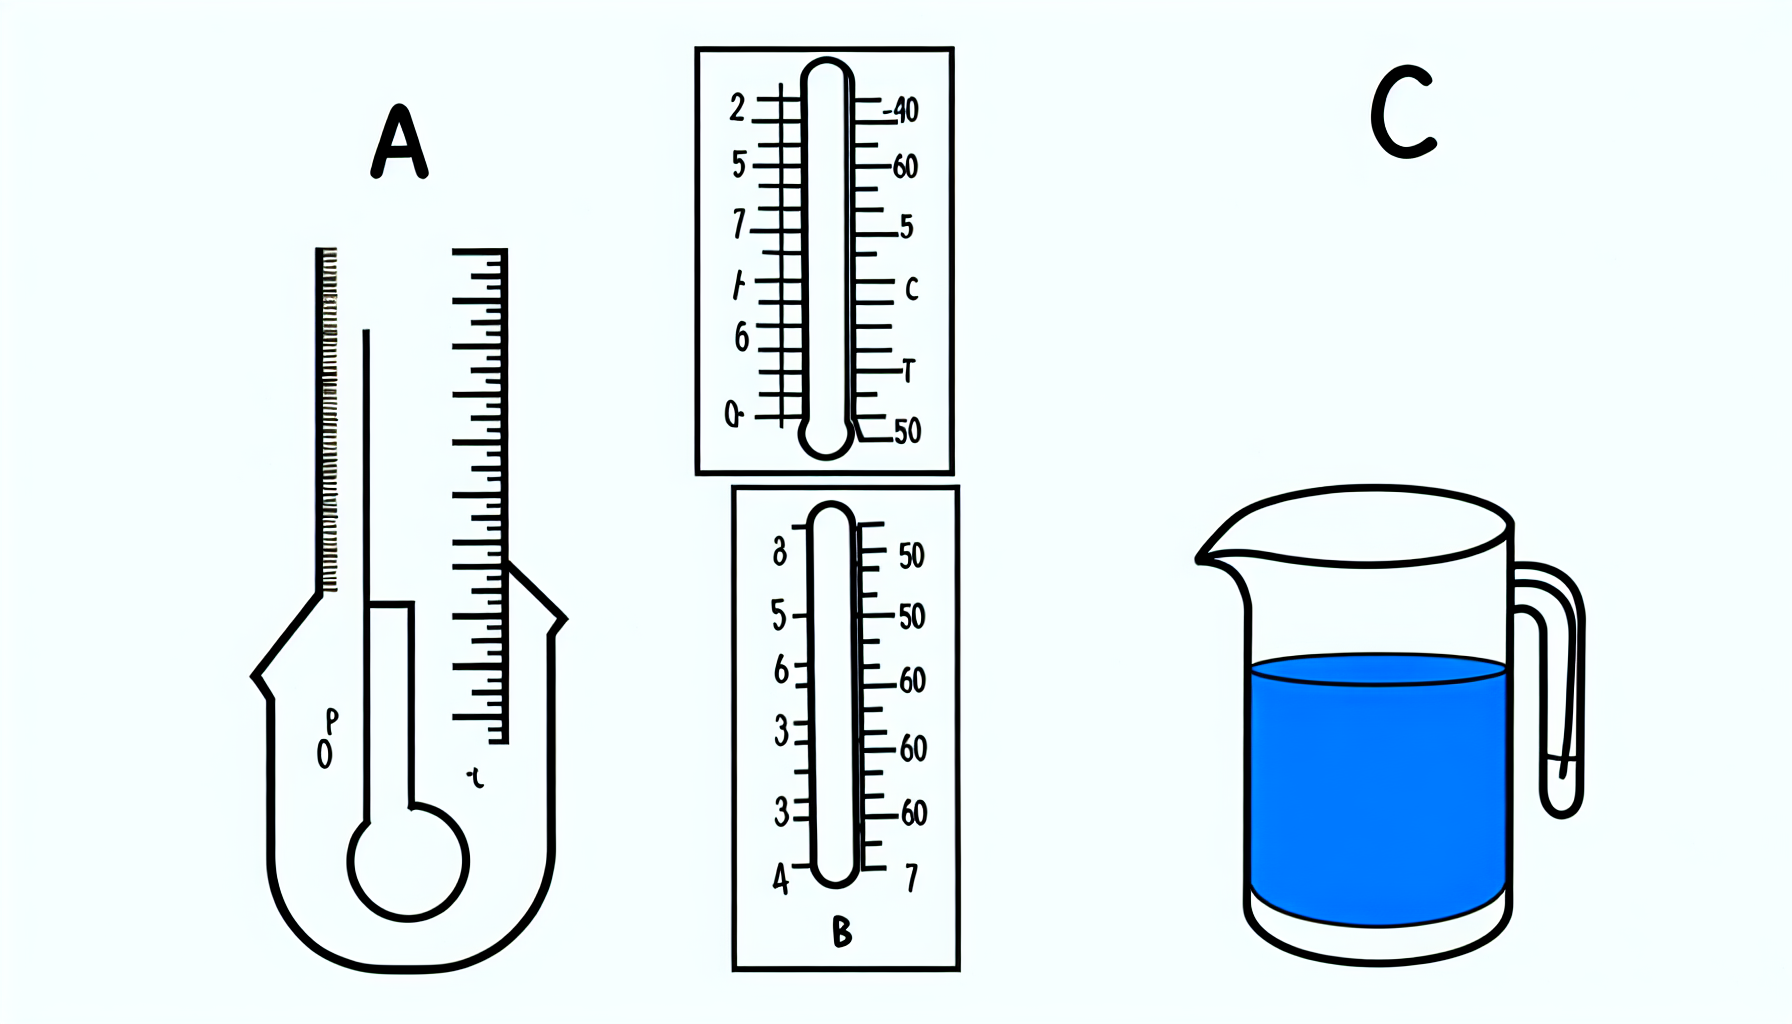
\includegraphics[width=0.88\textwidth,height=0.20\textheight,keepaspectratio]{visuals/lo-yr9-reading-scales-foundation-p1.png}
\end{center}
\vspace{0.02em}
\begin{columns}[T,onlytextwidth]
\begin{column}{0.32\textwidth}\MMProblem{1}{Read the thermometer. What value does it show?}\end{column}
\begin{column}{0.32\textwidth}\MMProblem{2}{Read the ruler. What value does it show?}\end{column}
\begin{column}{0.32\textwidth}\MMProblem{3}{Read the jug. What value does it show?}\end{column}
\end{columns}
\vspace{0.2em}
\begin{columns}[T,onlytextwidth]
\begin{column}{0.32\textwidth}\MMProblem{4}{Read the dial scale. What value does it show?}\end{column}
\begin{column}{0.32\textwidth}\MMProblem{5}{Read the speedometer. What value does it show?}\end{column}
\begin{column}{0.32\textwidth}\MMProblem{6}{Read the protractor. What value does it show?}\end{column}
\end{columns}
\vspace{0.2em}
\begin{columns}[T,onlytextwidth]
\begin{column}{0.32\textwidth}\MMProblem{7}{Read the pressure gauge. What value does it show?}\end{column}
\begin{column}{0.32\textwidth}\MMProblem{8}{Read the kitchen scale. What value does it show?}\end{column}
\begin{column}{0.32\textwidth}\MMProblem{9}{Read the thermometer. What value does it show?}\end{column}
\end{columns}
\end{frame}

\begin{frame}[t,shrink=15]
\WorksheetTitle{Start Tasks}{1}
\vspace{-0.10em}
\begin{center}
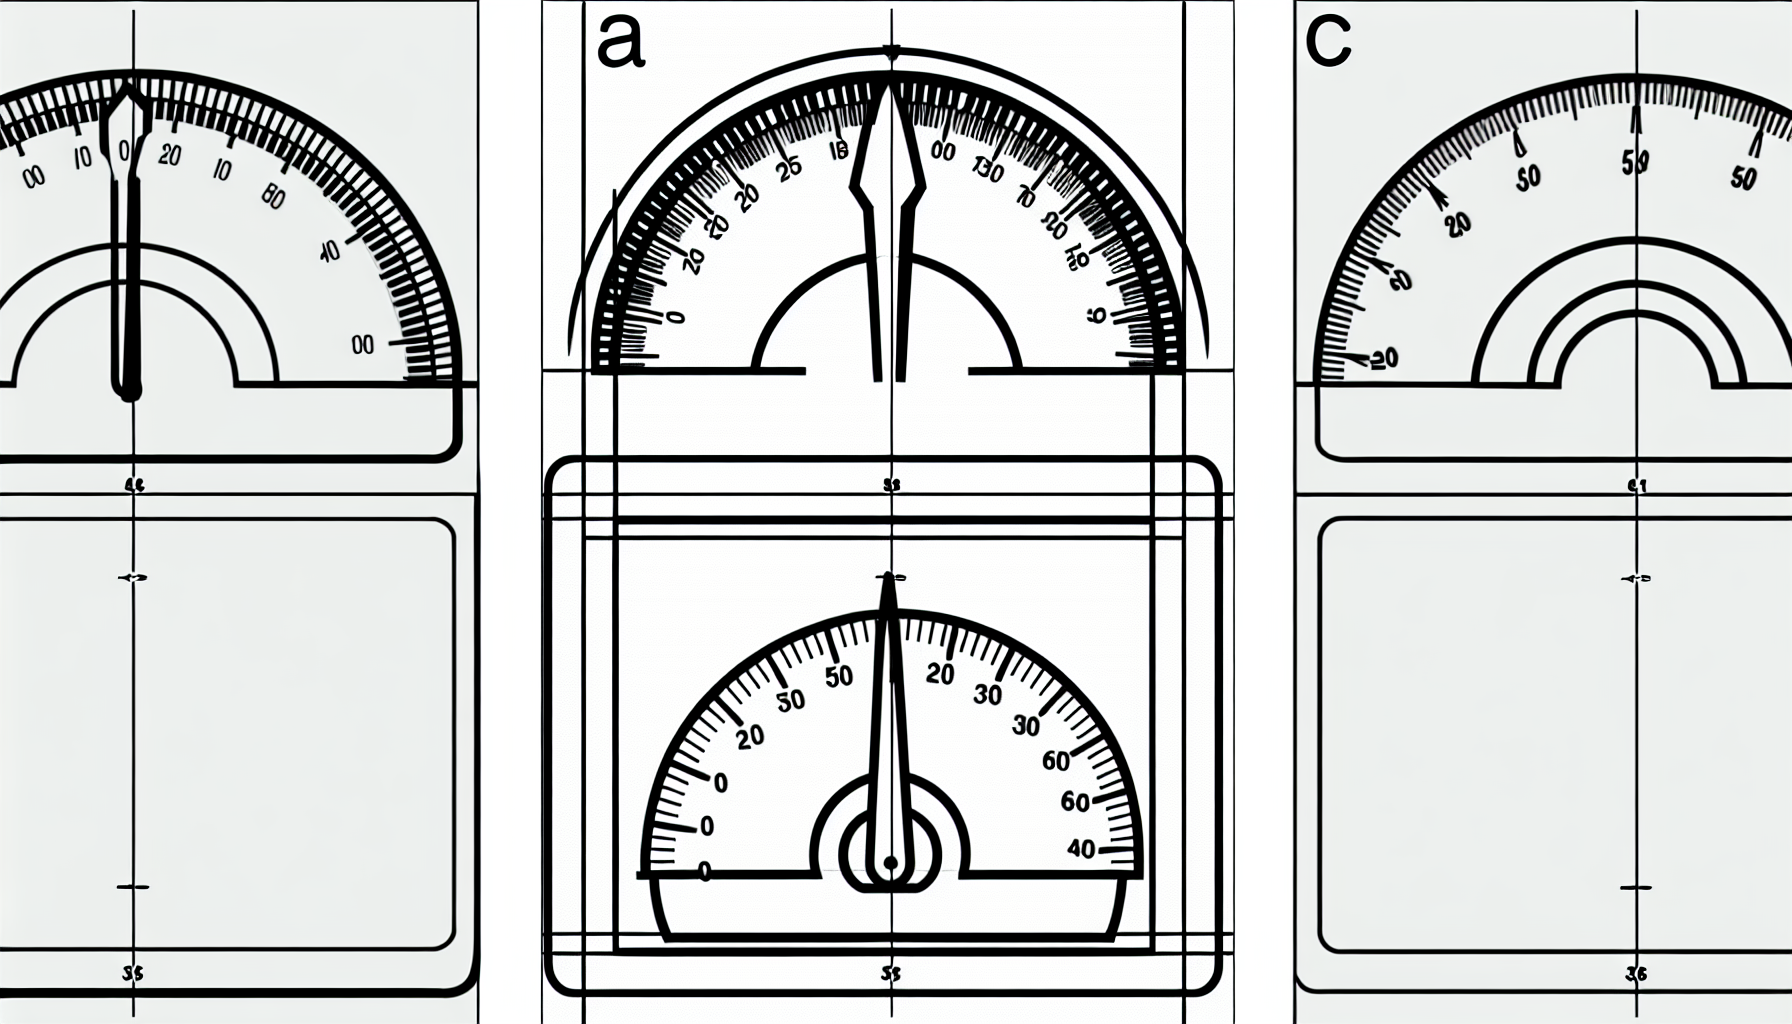
\includegraphics[width=0.88\textwidth,height=0.20\textheight,keepaspectratio]{visuals/lo-yr9-reading-scales-foundation-p2.png}
\end{center}
\vspace{0.02em}
\begin{columns}[T,onlytextwidth]
\begin{column}{0.32\textwidth}\MMProblem{10}{Read the ruler. What value does it show?}\end{column}
\begin{column}{0.32\textwidth}\MMProblem{11}{Read the jug. What value does it show?}\end{column}
\begin{column}{0.32\textwidth}\MMProblem{12}{Read the dial scale. What value does it show?}\end{column}
\end{columns}
\vspace{0.2em}
\begin{columns}[T,onlytextwidth]
\begin{column}{0.32\textwidth}\MMProblem{13}{Read the speedometer. What value does it show?}\end{column}
\begin{column}{0.32\textwidth}\MMProblem{14}{Read the protractor. What value does it show?}\end{column}
\begin{column}{0.32\textwidth}\MMProblem{15}{Read the pressure gauge. What value does it show?}\end{column}
\end{columns}
\vspace{0.2em}
\begin{columns}[T,onlytextwidth]
\begin{column}{0.32\textwidth}\MMProblem{16}{Read the kitchen scale. What value does it show?}\end{column}
\begin{column}{0.32\textwidth}\MMProblem{17}{Read the thermometer. What value does it show?}\end{column}
\begin{column}{0.32\textwidth}\MMProblem{18}{Read the ruler. What value does it show?}\end{column}
\end{columns}
\end{frame}

\begin{frame}[t,shrink=15]
\WorksheetTitle{Start Tasks}{1}
\vspace{-0.10em}
\begin{center}
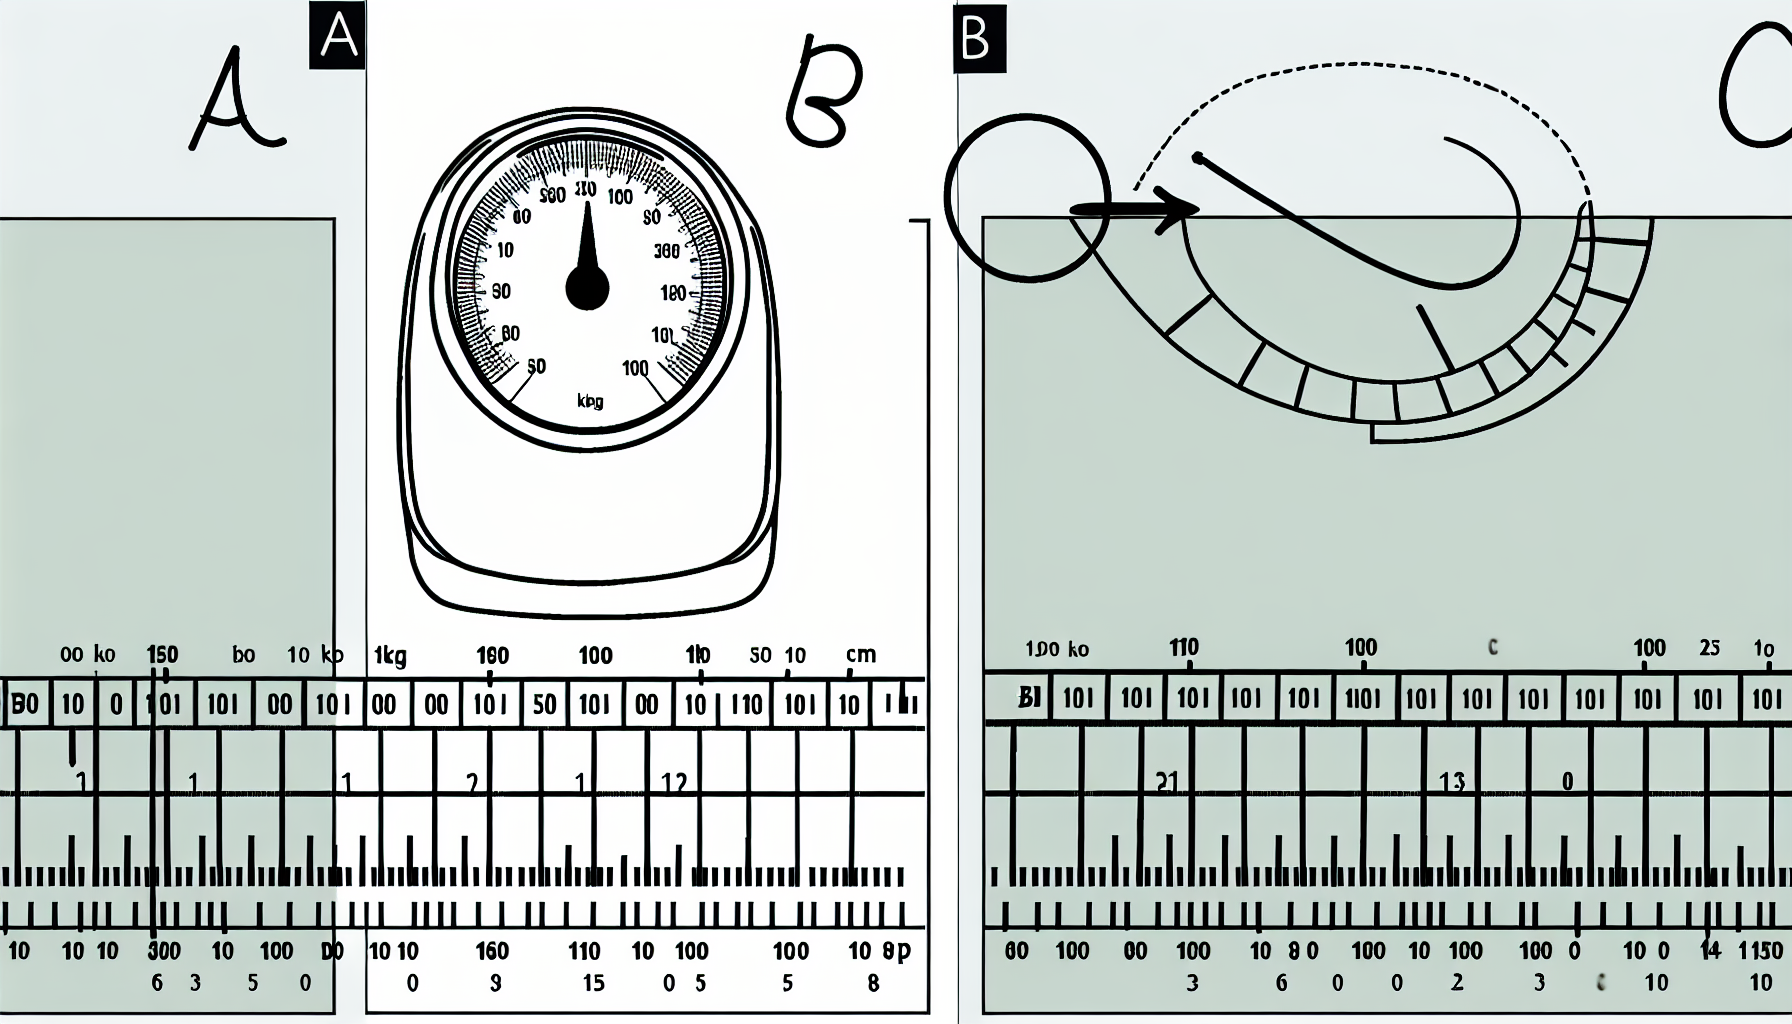
\includegraphics[width=0.88\textwidth,height=0.20\textheight,keepaspectratio]{visuals/lo-yr9-reading-scales-foundation-p3.png}
\end{center}
\vspace{0.02em}
\begin{columns}[T,onlytextwidth]
\begin{column}{0.32\textwidth}\MMProblem{19}{Read the jug. What value does it show?}\end{column}
\begin{column}{0.32\textwidth}\MMProblem{20}{Read the dial scale. What value does it show?}\end{column}
\begin{column}{0.32\textwidth}\MMProblem{21}{Read the speedometer. What value does it show?}\end{column}
\end{columns}
\vspace{0.2em}
\begin{columns}[T,onlytextwidth]
\begin{column}{0.32\textwidth}\MMProblem{22}{Read the protractor. What value does it show?}\end{column}
\begin{column}{0.32\textwidth}\MMProblem{23}{Read the pressure gauge. What value does it show?}\end{column}
\begin{column}{0.32\textwidth}\MMProblem{24}{Read the kitchen scale. What value does it show?}\end{column}
\end{columns}
\vspace{0.2em}
\begin{columns}[T,onlytextwidth]
\begin{column}{0.32\textwidth}\MMProblem{25}{Read the thermometer. What value does it show?}\end{column}
\begin{column}{0.32\textwidth}\MMProblem{26}{Read the ruler. What value does it show?}\end{column}
\begin{column}{0.32\textwidth}\MMProblem{27}{Read the jug. What value does it show?}\end{column}
\end{columns}
\end{frame}
\end{document}
